\section{Graphs}

\subsection{Laplacian of a graph \texorpdfstring{{\cite[Sec. 1.2]{chung_lectures_nodate}}}{[Chu, Sec. 1.2]}}

In a graph $G$, let $d_v$ denote the degree of the vertex $v$. We first define the Laplacian for graphs without loops and multiple edges. To begin, we consider the matrix $L$, defined as follows:
\[
L(u,v) = \begin{cases}
    d_v &\text{if } u = v \\
    -1 &\text{if $u$ and $v$ are adjacent}, \\
    0 & \text{otherwise}.
\end{cases}
\]
Let $T$ denote the diagonal matrix with the $(v,v)$-th entry having value $d_v$. The \defini{Laplacian} of $G$ is defined to be the matrix
\[
\mathcal{L}(u,v) = \begin{cases}
    1 & \text{if $u = v$ and $d_v \not= 0$} \\
    - \displaystyle\frac{1}{\sqrt{d_u \, d_v}} & \text{if $u$ and $v$ are adjacent}, \\
    0 & \text{otherwise}. 
\end{cases}
\]
We can write
\[
\mathcal{L} = T^{-1/2} \, L \, T^{-1/2}
\]
with the convention $T^{-1}(v,v) = 0$ for $d_v = 0$. We say $v$ is an isolated vertex if $d_v = 0$. A graph is said to be nontrivial if it contains at least one edge. The Laplacian $\mathcal{L}$ can be viewed as an operator on the space of functions $\fonctionens[g]{V(G)}{\R}$ which satisfies
\[
\mathcal{L}g(u) = \frac{1}{\sqrt{d_u}} \sum_{v \sim u} \left( \frac{g(u)}{\sqrt{d_u}} - \frac{g(v)}{\sqrt{d_v}} \right).
\]
When $G$ is $k$-regular, it is easy to see that
\[
\mathcal{L} = \I - \frac{1}{k} \, A,
\]
where $A$ is the adjacency matrix of $G$ and $\I$ is an identity matrix. All matrices here are $n \times n$ where $n$ is the number of vertices of $G$. 

For a general graph, we have
\[
    \mathcal{L} = T^{-1/2} \, L \, T^{-1/2} = \I - T^{-1/2} \, A \, T^{-1/2}.
\]
(lien avec la théorie de l'homologie)

\subsection{Eigenvalues of a graph \texorpdfstring{{\cite[Sec. 1.2]{chung_lectures_nodate}}}{[Chu, Sec. 1.4]}}

Since $\mathcal{L}$ is symmetric, its eigenvalues are all real and non-negative. We can use the variational characterizations of those eigenvalues in terms of the Rayleigh quotient of $\mathcal{L}$. Let $g$ denote an arbitrary function which assigns to each vertex $v$ of $G$ a real value $g(v)$. We can view $g$ as a column vector. Then
\begin{align}
    \frac{\crodua{g}{\mathcal{L}g}}{\crodua{g}{g}} &= \frac{\crodua{g}{T^{-1/2} L T^{-1/2} g}}{\crodua{g}{g}} \nonumber \\
    &= \frac{\crodua{f}{Lf}}{\crodua{T^{1/2} f}{T^{1/2} f}} \nonumber \\
    &= \frac{\sum\limits_{u \sim v} \big( f(u) - f(v) \big)^2}{\sum_v f(v)^2 \, d_v} \label{eq:rayleigh_quotient}
\end{align}
where $g = T^{1/2} f$ and $\sum\limits_{u \sim v}$ denotes the sum over all unordered pairs $\{u, v\}$ for which $u$ and $v$ are adjacent. Here $\crodua{f}{g} = \sum\limits_x f(x) \, g(x)$ denotes the standard inner product in $\R^n$. The sum $\sum\limits_{u \sim v} \big( f(u) - f(v) \big)^2$ is sometimes called the \defini{Dirichlet sum} of $G$ and the ratio on the left-hand side of \ref{eq:rayleigh_quotient} is often called the \defini{Rayleigh quotient}. 

From equation \ref{eq:rayleigh_quotient}, we see that all eigenvalues are non-negative. In fact, we can easily deduce from equation \ref{eq:rayleigh_quotient} that $0$ is an eigenvalue of $\mathcal{L}$. We denote the eigenvalues of $\mathcal{L}$ by $0 = \lambda_0 \leqslant \lambda_1 \leqslant \cdots \leqslant \lambda_{n-1}$. The set of the $\lambda_i$'s is called the \defini{spectrum} of $\mathcal{L}$. Let $\indicatrice$ denote the constant function which assumes the value $1$ on each vertex. Then $T^{1/2} \indicatrice$ is an eigenfunction of $\mathcal{L}$ with eigenvalue $0$. Furthermore,
\begin{equation} \label{eq:lambdaG}
    \boxed{
    \lambda_G = \lambda_1 = \inf_{f \perp T \indicatrice} \frac{\sum\limits_{u \sim v} \big( f(u) - f(v) \big)^2}{\sum_v f(v)^2 \, d_v}
    }.
\end{equation}
($f$ ranges over functions defined on the vertices of $G$ satisfying $\sum_v f(v) \, d_v = 0$). The corresponding eigenfunction is $g = T^{1/2} f$ as in \ref{eq:rayleigh_quotient}. The spectral gap $\lambda_G$ is the least nonzero eigenvalue of $\mathcal{L}$.

The above formulation for $\lambda_G$ corresponds in a natural way to the eigenvalues of the Laplace--Beltrami operator for Riemannian manifolds:
\[
\lambda_M = \inf_{\int_M f = 0} \frac{\int_M \abs{\grad f}^2}{\int_M \abs{f}^2}.
\]
We remark that the corresponding measure here for each edge is $1$. The measure for each vertex is the degree of the vertex.

We note that \ref{eq:lambdaG} also has the formulation
\[
\boxed{
\lambda_G = \lambda_1 = \inf_f \frac{\sum\limits_{u \sim v} \big( f(u) - f(v) \big)^2}{\sum\limits_v \big( f(v) - \overline{f} \big)^2 \, d_v},
\quad
\text{where}
\quad
\overline{f} = \frac{\sum_v f(v) \, d_v}{\vol G}
},
\]
and $\vol G$ denotes the volume of the graph $G$, given by $\vol G = \sum\limits_v d_v$. More generally, for a set $S$, the volume of $S$, denoted by $\vol(S)$ is defined to be $\vol(S) \defeq \sum_{v \in S} d_v$.

\subsection{Cheeger inequality on graphs \texorpdfstring{{\cite[Sec. 2]{ji_fourth_2010}}}{[Ji+10, Sec. 2]}}

For a set $S$, the \defini{Cheeger ratio} of $S$ is defined to be
\[
h_S \defeq \frac{\abs{\partial S}}{\min\{ \vol(S), \vol(G) - \vol(S) \}},
\]
where the boundary of $S$ is denoted $\partial S \defeq \ens[\big]{ \{u, v\} \in E \tq u \in S \text{ and } v \not\in S }$.  Let $\overline{S}$ denote the complement of $S$. Then $h_S = h_{\overline{S}}$. The \defini{Cheeger constant} of $G$ is denoted by
\[
h_G \defeq \min_S h_S.
\] 

\begin{figure}[H]
    \centering
    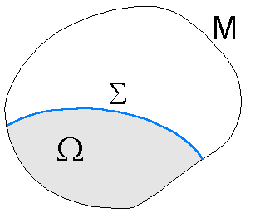
\includegraphics[width=0.3\textwidth]{img/isoperimetric-problem-in-a-region.png}
    \caption{}
\end{figure}

\begin{theo}[Cheeger inequality {\cite[Theo. 1]{ji_fourth_2010}}] \label{theo:cheeger_inequality}
In a graph $G$, the Cheeger constant $h_G$ and the \defini{spectral gap} $\lambda_G$ are related as follows:
\[
2 \, h_G \geqslant \lambda_G \geqslant \frac{\alpha_G{}^2}{2} \geqslant \frac{h_G{}^2}{2}
\]
where $\alpha_G$ is the minimum Cheeger ratio of subsets $S_i$ consisting of vertices {\color{red} with the largest $i$ values in the eigenvector} associated with $\lambda_G$, over all $i$. 
\end{theo}

\begin{demo}
For a proof of the Cheeger inequality using  eigenvectors, see \cite[Sec. 3]{ji_fourth_2010}.
\end{demo}